\documentclass[journal]{IEEEtran}
\usepackage[T1]{fontenc}
\usepackage{amsmath,amssymb,amsfonts}
\usepackage{graphicx}
\usepackage{booktabs}
\usepackage{multirow}
\usepackage{siunitx}
\usepackage{xcolor}
\usepackage{url}
\usepackage[hidelinks]{hyperref}
\usepackage{tikz}
% Shared TikZ style for every project diagram (README figures and the manuscript).
\usepackage{amsmath,amssymb}
\usetikzlibrary{arrows.meta,positioning,fit,backgrounds,calc,shapes.geometric,decorations.pathreplacing}
\definecolor{cam}{HTML}{2563EB}     % endoscope / camera action
\definecolor{armA}{HTML}{EA580C}    % instrument arm USM1
\definecolor{armB}{HTML}{16A34A}    % instrument arm USM3
\definecolor{armC}{HTML}{9333EA}    % instrument arm USM4
\definecolor{ink}{HTML}{1F2937}
\definecolor{muted}{HTML}{6B7280}
\definecolor{panel}{HTML}{F3F4F6}
\definecolor{model}{HTML}{0F766E}
\tikzset{
  >={Stealth[length=2.2mm]},
  every node/.style={font=\sffamily\small, text=ink},
  box/.style={draw=ink!60, rounded corners=2pt, fill=white, inner sep=4pt, align=center, line width=0.5pt},
  data/.style={box, fill=panel},
  proc/.style={box, fill=model!8, draw=model!70},
  learn/.style={box, fill=model!20, draw=model, line width=0.8pt},
  sig/.style={box, font=\sffamily\scriptsize},
  group/.style={draw=muted!70, dashed, rounded corners=4pt, inner sep=6pt},
  flow/.style={->, line width=0.7pt, draw=ink!70},
  note/.style={font=\sffamily\scriptsize, text=muted, align=center},
  token/.style={draw, rounded corners=1pt, minimum width=5mm, minimum height=4mm, inner sep=1pt,
                font=\sffamily\scriptsize\bfseries},
}

\graphicspath{{../../docs/figures/}}
\newcommand{\todo}[1]{\textcolor{red}{[#1]}}
\newcommand{\method}{EG-SWM}
% Result numbers in the text come from scripts/eval/aggregate.py (tables/numbers.tex); a missing key prints ??
\newcommand{\val}[1]{\ifcsname val@#1\endcsname\csname val@#1\endcsname\else\textcolor{red}{\textbf{??}}\fi}
\InputIfFileExists{tables/numbers}{}{}

\begin{document}
\title{Embodiment-Grounded Surgical World Models:\\ Learning Arm-Factorized, Camera-Aware Actions from Unlabeled Robotic Video}
% TODO(authors): author list and affiliations to be provided by the corresponding author.
\author{Ajo~Babu~George%
\thanks{\todo{Affiliations, funding and acknowledgements.}}}

\markboth{IEEE Transactions on Medical Robotics and Bionics}{George \MakeLowercase{\textit{et al.}}: Embodiment-Grounded Surgical World Models}
\maketitle

\begin{abstract}
World models that predict how the operative scene evolves under a robot's actions could serve surgical robotics as simulators, policy evaluators and data generators. Current surgical world models either require synchronized robot kinematics, which exist for only a few hundred hours of laboratory data, or learn a single latent action from unlabeled video that must explain endoscope motion, several instruments and tissue response at once. We observe that the embodiment of a teleoperated surgical robot is visible even when its kinematics are not: system logs record which arm carries the endoscope and which instrument is mounted on every other arm, and the console overlay shows which arms the surgeon drives. We present \method{}, a world model whose action space mirrors the robot: an explicit endoscope ego-motion action and one latent action per instrument arm, inferred by an inverse-dynamics model that only observes the arm's own instrument region, bound to arms through the robot log. A latent spatio-temporal diffusion transformer trained with rectified flow and per-frame noise levels predicts future endoscopic video from context frames and these actions. Trained on 476\,h of in-vivo da Vinci video from 123 cases without any kinematic labels and compared with other action interfaces at equal capacity, data and budget, \method{} is the only one that keeps the endoscope and each instrument controllable and still predicts better than a copied frame. Frame-wide latent actions (monolithic, slots) predict \val{diff/S_global-S_arms/psnr}--\val{diff/S_slots-S_arms/psnr}\,dB better but take over the endoscope motion, realising only \val{ctl/S_slots/gain_pct}--\val{ctl/S_global/gain_pct}\,\% of a commanded endoscope move against \val{ctl/S_arms/gain_pct}\,\% for \method{}; among the controllable interfaces, \method{} leads twelve discrete latent actions by \val{diff/S_arms-S_global_vq/psnr}\,dB and robot-state conditioning by \val{diff/S_arms-S_state/psnr}\,dB. On held-out episodes of three public datasets with da Vinci kinematics, a linear probe on its frozen arm actions explains \val{kin/mean/S_arms/pos} of the variance of the same arm's end-effector translation (monolithic latent: \val{kin/mean/S_global/pos}), and initialising kinematics-conditioned models from \method{} changes their PSNR on SutureBot and SRT-H by \val{e3/suturebot/arms/0.1/vs_scratch} and \val{e3/srth/arms/0.1/vs_scratch}\,dB when only 10\,\% of the training episodes are available. We release code, processed annotations and weights.
\end{abstract}

\begin{IEEEkeywords}
Surgical robotics, world models, video prediction, latent actions, robot-assisted surgery, generative models.
\end{IEEEkeywords}

\section{Introduction}
\IEEEPARstart{A}{world} model predicts how an environment evolves in response to an agent's actions. In robot-assisted surgery such a model could act as a photorealistic simulator for training and planning, as an automatic evaluator of autonomous policies \cite{cosmossurgdvrk}, and as a generator of paired video--action data for learning those policies \cite{cosmoshsurg,surgwam}. Medical world models have begun to show this value outside surgery, for example by simulating tumour response to candidate treatments and choosing among them \cite{mewm}.

Building surgical world models is limited by the action signal. Models conditioned on robot kinematics \cite{openh,kvlr,surgcast,surgwam} can be precisely controlled, but synchronized kinematics are recorded only on research platforms such as the da Vinci Research Kit, mostly on phantoms or ex-vivo tissue, totalling a few hundred hours across all public datasets \cite{openh}. Clinical and in-vivo robotic video is far more abundant but carries no kinematics. Action-free approaches learn latent actions from such video in the manner of Genie \cite{genie}: the surgical vision world model of Koju et al.\ \cite{surgwm} infers one of twelve discrete latent actions per frame transition. A single, monolithic latent action, however, has to explain everything that changes between two endoscopic frames---endoscope motion, the motion of two or three instruments, and the tissue's response---and latent-action learning is known to degrade sharply under such action-correlated distractors unless a small amount of supervision is added \cite{laom}.

We start from an observation about teleoperated surgical robots: \emph{their embodiment is observable even when their kinematics are not}. The da Vinci system logs which of its four arms holds the endoscope and which instrument is mounted on every other arm, with timestamps; the console overlay burned into the recorded video shows which arms the surgeon's hands currently drive and when energy is applied; and teleoperation itself is structured, because at most two instrument arms move at once and the endoscope moves in a separate control mode. These signals come for free with thousands of hours of video, yet no surgical world model uses them.

We propose \method{}, an embodiment-grounded surgical world model whose action space mirrors the robot (Fig.~\ref{fig:arch}). The endoscope action is explicit: a four-parameter similarity transform measured from the video itself. Each instrument arm receives its own latent action, inferred by an inverse-dynamics model that observes only that arm's instrument region---located by an instrument detector and bound to the arm through the robot log---and constrained by an information bottleneck. A latent spatio-temporal diffusion transformer predicts future video tokens from context frames, the endoscope action through adaptive normalization, and one token per arm through cross-attention. Because each action is tied to a physical actuator, the model can be steered one arm at a time and its actions can be compared with real kinematics.

Our contributions are:
\begin{itemize}
\item \method{}, to our knowledge the first surgical world model with an embodiment-factorized action space learned without kinematic labels, combining an explicit endoscope ego-motion action with per-arm latent actions grounded in robot system logs.
\item A data pipeline that turns \todo{838}\,h of in-vivo da Vinci video and its system logs into model-ready windows with robot state, endoscope ego-motion and arm-bound instrument regions, and an analysis of the label noise in such logs.
\item An evaluation protocol for surgical world models that goes beyond pixel fidelity: controllability, per-arm locality, compliance with commanded endoscope motion, consistency of the predicted scene with the robot's state, and linear probing of learned actions against real kinematics.
\item Extensive experiments against monolithic \cite{genie,surgwm} and factored \cite{flam} latent actions at equal capacity, kinematics-conditioned baselines \cite{openh} on public benchmarks, and ablations of every component. They show that fidelity and control pull apart: an action that covers the whole frame predicts better because it absorbs the endoscope motion, whereas actions bound to the robot's arms keep each actuator controllable at a small cost in fidelity, concentrated where instruments are not bound to an arm. \todo{Kinematic grounding and transfer findings.}
\end{itemize}

\section{Related Work}
\subsection{Surgical video generation}
Diffusion and transformer models now generate realistic endoscopic video. Unconditional or text-conditioned models include Endora \cite{endora}, SurGen \cite{surgen}, Bora \cite{bora}, Ophora \cite{ophora} and the hierarchy-aware HieraSurg \cite{hierasurg}; FLAIR learns action priors from optical flow and injects them into a frozen backbone \cite{flair}. Structure-conditioned models steer generation with action graphs \cite{visage}, optical flow and user trajectories \cite{surgsora}, sparse masks \cite{surgiflowvid}, tool-tip trajectories with tissue affordances \cite{saw} or multimodal control experts \cite{suruniworld}. These models produce convincing appearance, but their controls describe pixels rather than the robot, and expert assessment shows that visual plausibility does not imply plausible instrument operation or tissue response \cite{surgveo}.

\subsection{Surgical world models}
Kinematics-conditioned world models predict endoscopic video from robot actions. Cosmos-H-Surgical fine-tunes a physical-AI foundation model and uses an inverse-dynamics model to label synthetic video for policy learning \cite{cosmoshsurg}; Open-H-Embodiment provides the largest open corpus of medical robot video with kinematics and an action-conditioned simulator trained on it \cite{openh}, later distilled for real-time use \cite{cosmoshdreams} and applied to policy evaluation \cite{cosmossurgdvrk}. KVLR lifts articulated kinematics to image-aligned control maps \cite{kvlr}, SurgCast predicts future instrument skeletons \cite{surgcast}, and world-action models jointly predict video and robot actions \cite{surgwam,endowam,jointvt}. Other work targets long-horizon drift \cite{surgvista}, hierarchical event structure \cite{s2hwm}, failure detection \cite{fomofd} and motion-centric benchmarks \cite{surgwmbench}. All of these need kinematics for training or control. The surgical vision world model of Koju et al.\ \cite{surgwm} is the closest action-free approach: it applies the Genie recipe \cite{genie} to SurgToolLoc video at $120\times180$ pixels and 1\,fps with twelve discrete latent actions. Its successor SurgTransfer infers one continuous latent action per frame, relative to the first frame of the clip, and conditions a fine-tuned Stable Video Diffusion model on it \cite{surgtransfer}; both keep a single action for the whole frame.

\subsection{Latent actions and factorization}
Latent action models infer actions from unlabeled video by inverse dynamics and train a forward model on them \cite{genie,lapa,adaworld,villax}. Nikulin et al.\ show that such latents collapse when distractors correlate with the true actions and that a little action supervision during latent-action learning restores them \cite{laom}; object-centric decomposition \cite{oclam} and factored latent actions with one action per learned scene factor \cite{flam} reduce the problem in multi-entity scenes. Factoring out camera ego-motion makes motion targets comparable across moving and static cameras \cite{egowam}, and EndoWorld-JEPA separates dominant displacement from residual motion for endoscopic representation learning \cite{endoworldjepa}. Closest to our goal, SkeLAM splits a robot's latent action into a kinematic component, supervised by renderings of the robot's skeleton computed from its joint states, and a residual component that keeps the rest of the transition, and conditions a robot world model on both \cite{skelam}. EXE factorizes action labels, estimated hand poses and robot end-effector poses, into a positional subspace shared across embodiments and embodiment-specific codebooks for policy pretraining \cite{exe}. A controlled study of latent actions for policy learning finds that the strength of the bottleneck matters more than its form, and that linear probes rank latent actions only coarsely \cite{lamstudy}. \method{} differs in that its factors are not discovered but defined by the robot, and need neither kinematics nor action labels: one explicit endoscope action and one latent per instrument arm, bound to arms by the robot's own logs. Our scene-action variant plays the role of SkeLAM's residual, and we find that it takes over part of the endoscope motion (Section~\ref{sec:results}).

\subsection{Diffusion world models}
Our dynamics model follows diffusion and flow-matching transformers \cite{dit,pixartalpha,rectflow,flowmatching,sd3} trained with per-frame noise levels as in Diffusion Forcing \cite{dforcing}, which supports autoregressive rollout; related designs underlie game and robot world models \cite{diamond,unisim,cosmos,cosmospredict25} and video foundation models \cite{wan}.

\section{Data and Embodiment Signals}\label{sec:data}
\subsection{In-vivo robotic video with robot logs}
We use the SurgVU corpus \cite{surgvu}: 155 porcine training-laboratory cases recorded on da Vinci Xi systems, 280 video files totalling 837.8\,h at $1280\times720$ and 60\,fps. Each case comes with the system log of its four universal surgical manipulators (USM1--4): install and uninstall times of every instrument \emph{and of the endoscope}, and with task segments from a training curriculum (218\,h annotated; 7 tasks, 46 curriculum topics). After removing black, out-of-body and blank footage, about 604\,h are usable (Fig.~\ref{fig:pipeline}). Cases are split into 123 training, 12 validation and 20 test cases, stratified by endoscope arm, case length and dominant task.

The logs record part-relative times; converted to a single case timeline they give, at every instant, the robot configuration $s_t=(o^1_t,\dots,o^4_t)$ with $o^k_t$ the occupant of arm $k$ (empty, endoscope, or one of 20 instrument types). The endoscope is moved between ports in most cases (211 port changes in 104 of 155 cases), so the camera arm is itself part of the time-varying state; three instruments are mounted 65\,\% of the time and instruments are exchanged 7.1 times per hour. The logs are noisy: 97\,\% of overlapping intervals on one arm are stale intervals left by missing uninstall events, which we resolve by letting the most recent installation win.

\begin{figure*}[t]
\centering
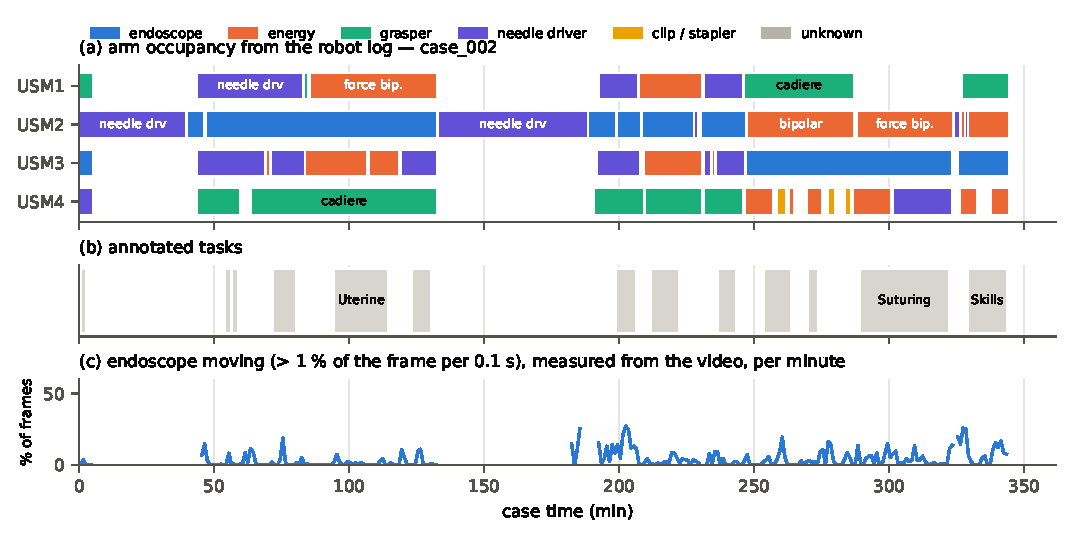
\includegraphics[width=\textwidth]{embodiment_timeline.pdf}
\caption{The robot's embodiment is observable without kinematics. One training case: (a) arm occupancy from the system log (the endoscope changes ports and instruments are exchanged on every arm), (b) annotated curriculum tasks, (c) share of frames per minute in which the endoscope moves, measured from the video.}
\label{fig:embodiment}
\end{figure*}

\subsection{Console overlay}
The surgeon console renders a status band over the recorded video on 81\,\% of usable frames. Per arm it shows the mounted instrument, the endoscope, the hand (left/right) that currently drives the arm, and energy activation. We crop the band away before the model sees any pixel, so that the model cannot read instrument identities from the screen. The driving hand and energy activation of each arm, read from the band, are tested as additional conditioning (Section~\ref{sec:parts}).

\begin{figure*}[t]
\centering
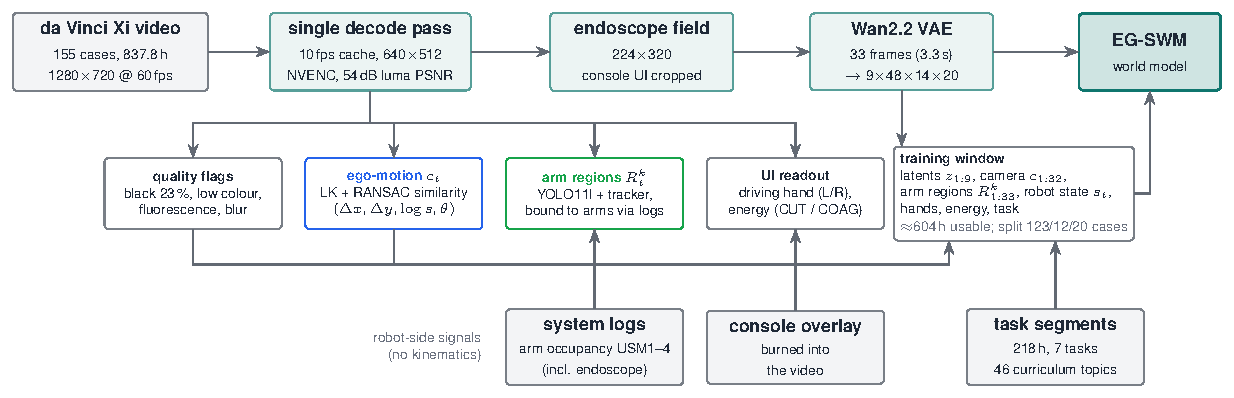
\includegraphics[width=\textwidth]{pipeline.pdf}
\caption{Data pipeline. One decode pass converts the in-vivo video into a 10\,fps cache with per-frame quality flags and endoscope ego-motion; instrument detections are bound to robot arms through the system log; the world model sees only the endoscope field encoded by a frozen video VAE.}
\label{fig:pipeline}
\end{figure*}

\section{Method}\label{sec:method}
\begin{figure*}[t]
\centering
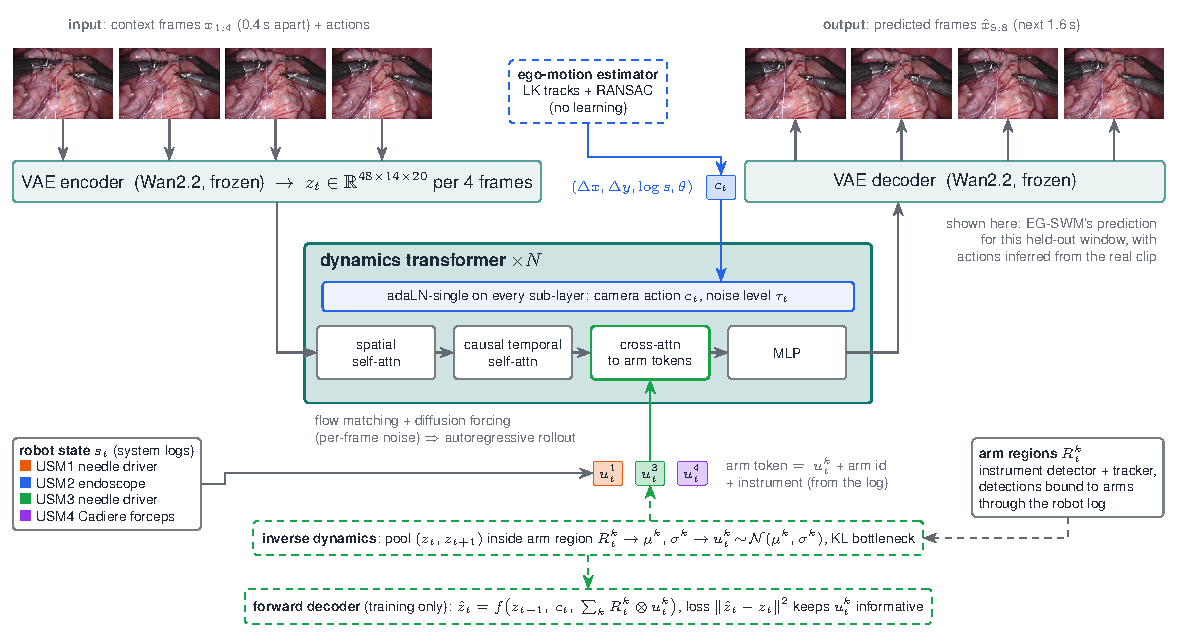
\includegraphics[width=\textwidth]{architecture.pdf}
\caption{\method{}. Context frames are encoded by a frozen video VAE; a latent spatio-temporal diffusion transformer predicts future latents conditioned on an explicit endoscope ego-motion action (through AdaLN) and on one token per robot arm (through cross-attention) that carries the arm's identity, its logged instrument and a latent action inferred from that arm's instrument region. In training only, a forward decoder predicts each latent from its predecessor and the actions placed on their regions, which keeps the learned actions informative. Sample input and output from a held-out test case.}
\label{fig:arch}
\end{figure*}

\subsection{Overview}
Let $x_{0:32}$ be 33 consecutive endoscopic frames (3.3\,s at 10\,fps) of the endoscope field, resized to $224\times320$. A frozen causal video VAE \cite{wan} maps them to latents $z_{0:8}$, $z_t\in\mathbb{R}^{48\times14\times20}$, where $z_0$ encodes $x_0$ and $z_t$ ($t\ge1$) encodes frames $4t-3,\dots,4t$. The world model predicts $z_{n:8}$ from context $z_{0:n-1}$, the robot state $s_t$ and an action $a_t$ for every transition $z_{t-1}\to z_t$:
\begin{equation}
a_t=\big(c_t,\ \{u^k_t\}_{k\in\mathcal{K}_t}\big),
\end{equation}
where $c_t$ is the endoscope ego-motion and $u^k_t$ a latent action for each arm $k$ that carries an instrument.

\subsection{Endoscope action}
The endoscope is an arm of the robot that the surgeon commands, so we treat its motion as an explicit action. For consecutive frames we track Shi--Tomasi corners \cite{shitomasi} with pyramidal Lucas--Kanade \cite{lucaskanade}, discard tracks failing a forward--backward check, and fit a similarity transform with RANSAC \cite{ransac}; instruments move independently of the camera and are rejected as outliers. Each transition yields $(\Delta x,\Delta y,\log s,\theta)$ with translations measured at the image centre as fractions of the frame size. Because the endoscope is still most of the time and then moves quickly, we compress each parameter with a signed logarithm $\operatorname{sign}(c)\log(1+|c|/\sigma)$, $\sigma$ being its 90th percentile. A fit is unreliable when fewer than 12 tracks survive or the RANSAC inlier ratio is below 0.5 (12\,\% of transitions); its parameters are set to zero and a validity flag is cleared, so that ``not measured'' is not confused with ``endoscope still''. The four transitions inside a latent step and their flags form $c_t\in\mathbb{R}^{20}$.

\textbf{Validation.} On CRCD \cite{crcd}, which records the endoscope arm's joints, the estimate detects real endoscope motion with a ROC AUC of 0.81 per latent step (0.88 on steps whose four transitions are all reliable); horizontal translation, vertical translation and scale correlate with the yaw, pitch and insertion joints ($r=0.63$, $0.70$, $0.42$; sign agreement 81, 87 and 73\,\%), and the joint motion predicts the estimate with a leave-one-episode-out $R^2$ of 0.41. These figures use only episodes whose video and kinematics we verified to be synchronized (Sec.~\ref{sec:setup}). On AutoLaparo \cite{autolaparo}, 300 clips of human laparoscopic hysterectomy with an assistant-held laparoscope in which surgeons labelled the laparoscope move beginning at 5\,s (static, up, down, left, right, zoom in or out), the motion measured in the following second separates moves from static clips with a ROC AUC of 0.87; a rule with five parameters fitted on the official training clips classifies the test clips with 71\,\% accuracy (majority class 22\,\%) and gives 81\,\% of the moves their correct direction, with signs that follow the camera geometry.

\subsection{Arm-bound instrument regions}
A YOLO11 detector \cite{yolo11} trained for SurgVU instrument detection locates instrument tips at the boundary frame of every latent step. Detections are bound to arms by solving, per frame, an assignment problem \cite{hungarian} between the arms that carry an instrument and the detections, with cost
\begin{equation}
C_{kj}=-\log p_j+\lambda_c\,\mathbb{1}[\hat y_j\neq o^k_t]+\lambda_s\,\lVert \mathbf{m}_j-\boldsymbol{\mu}^k\rVert_2,
\end{equation}
where $p_j$ and $\hat y_j$ are the detection's confidence and class, $\mathbf{m}_j$ its centre, and $\boldsymbol{\mu}^k$ the typical image position of arm $k$ in this case, estimated from frames in which every mounted instrument type is unique. Assignments above a cost threshold are rejected. The region $R^k_t$ of arm $k$ at step $t$ is the union of its boxes at the two boundary frames of the step, rasterized onto the $14\times20$ latent grid and dilated by one cell.

\subsection{Per-arm latent actions}
An inverse-dynamics model (IDM) infers each arm's action from the latents it moves. A small transformer encodes every latent position of the transition, $F=\mathrm{Trunk}([z_{t-1},z_t,z_t-z_{t-1}])$. A query built from the arm's identity and logged instrument attends to $F$ \emph{only inside} $R^k_t$, and a head outputs a diagonal Gaussian:
\begin{equation}
(\boldsymbol\mu^k_t,\log\boldsymbol\sigma^{2,k}_t)=g\big(\mathrm{Attn}(q(k,o^k_t),F;\,R^k_t)\big),\quad u^k_t\sim\mathcal{N}(\boldsymbol\mu^k_t,\boldsymbol\sigma^{2,k}_t),
\end{equation}
with $u^k_t\in\mathbb{R}^{8}$. A Kullback--Leibler penalty towards $\mathcal{N}(0,I)$ bounds the information each action carries; arms without a visible instrument receive $u^k_t=0$. Restricting the evidence to the arm's own region prevents an arm's action from describing endoscope motion or another instrument, and binding through the log gives every action a fixed physical meaning across cases.

\subsection{Dynamics transformer}
The dynamics model is a latent spatio-temporal diffusion transformer. Latent positions become tokens; each block applies self-attention within a frame with 2-D rotary embeddings \cite{rope}, causal self-attention across frames at each position, cross-attention to the arm tokens of the frame, and a SwiGLU MLP. Arm $k$ at step $t$ contributes the token
\begin{equation}
e^k_t=W_u u^k_t+E_{\mathrm{arm}}[k]+E_{\mathrm{occ}}[o^k_t],
\end{equation}
with $o^k_t$ the occupant from the robot log. Adding the driving hand and energy activation read from the console overlay changes neither prediction nor control (Section~\ref{sec:parts}), so \method{} does without them. The noise level and the endoscope action modulate every sub-layer through adaptive normalization with a shared projection and per-block offsets \cite{pixartalpha}.

\subsection{Training objective}
We train with rectified flow \cite{rectflow,flowmatching}. Every latent frame has its own noise level $\tau_t\in[0,1]$, $x_t=(1-\tau_t)z_t+\tau_t\epsilon_t$, and the network predicts the velocity $\epsilon_t-z_t$:
\begin{equation}
\mathcal{L}=\mathbb{E}\Big[\sum_{t}w_t\big\lVert v_\theta(x,\tau,a,s)_t-(\epsilon_t-z_t)\big\rVert^2\Big]+\lambda\,\mathcal{L}_{\mathrm{fwd}}+\beta\sum_{t,k}\mathrm{KL}\big(q(u^k_t)\,\Vert\,\mathcal{N}(0,I)\big).
\end{equation}
Trained on the diffusion loss alone, the learned actions collapse to the prior: in a pilot run with $\beta=10^{-3}$, all eight action dimensions became inactive (KL $0.004$\,nats per arm) and replacing every arm's action with another clip's changed the loss by less than $0.01$\,\%, while replacing the explicit endoscope action raised it by up to 14\,\%. Presumably the diffusion model explains most of a transition from its context frames and the noisy target, so the few nats an action carries are not worth their KL cost. We therefore add a latent-action-model objective as in \cite{genie,lapa,adaworld}, grounded like the actions themselves: a small convolutional decoder $f$ with a $9\times9$-cell receptive field predicts each latent from its predecessor, the endoscope action and the arm actions placed on their regions,
\begin{equation}
\mathcal{L}_{\mathrm{fwd}}=\sum_t\big\lVert f\big(z_{t-1},c_t,\textstyle\sum_k R^k_t\otimes u^k_t\big)-z_t\big\rVert^2,
\end{equation}
where $R^k_t\otimes u^k_t$ writes $u^k_t$ into the channels of arm $k$ at the positions of its region. Instrument motion cannot be predicted locally without the actions, which keeps them informative while the diffusion model learns to use them. A weaker bottleneck alone is not enough (Section~\ref{sec:parts}). Baseline action interfaces receive the same decoder, with the monolithic or slot actions broadcast to every position. We use $\lambda=1$ and $\beta=10^{-4}$.
With probability 0.75 the first one to three latents are context ($\tau=0$, or $\tau\sim\mathcal{U}(0,0.1)$ to tolerate drift) and the remaining frames share one noise level or receive independent ones; otherwise all levels are independent, as in Diffusion Forcing \cite{dforcing}. Noise levels follow a logit-normal distribution \cite{sd3}, $w_t$ excludes context frames, and $\beta$ is ramped up over the first \num{10000} steps. With probability 0.1 all actions are dropped, which enables classifier-free guidance on actions.

\subsection{Inference}
Given context latents, future latents start from noise and are integrated with Euler steps from $\tau=1$ to $0$ while context latents stay fixed. Actions are either inferred from ground-truth video (\emph{action replay}, used to measure how well actions explain the future), taken from another clip (\emph{action swap}, to measure controllability), or set directly: an endoscope motion, or the action of a single arm. Longer rollouts re-anchor on the last generated frames.

\section{Experimental Setup}\label{sec:setup}
\subsection{Datasets and protocol}
\textbf{SurgVU} (in-vivo, no kinematics). Models are trained on all usable 3.3\,s windows of the 123 training cases and selected on the 12 validation cases. The test set is a fixed list of 1,900 windows, 100 drawn from each test case; fidelity is measured on 1,000 of them and the control and embodiment tests on 300, each spread evenly over the list so that every test case contributes. One of the 20 test cases is excluded: for 78\,\% of its windows the recorder shows colour bars (no video input), and the rest contains no surgery. Colour bars pass the usual frame filters, being bright, saturated and sharp; we detect them from the VAE latents, which are constant down every column (0.84\,\% of all windows). Two latents (0.5\,s, five frames) are given as context and the model predicts the remaining 2.8\,s.

\textbf{Kinematic grounding and transfer.} To test whether learned actions correspond to robot motion we use datasets with synchronized kinematics: JIGSAWS \cite{jigsaws} (da Vinci, bench-top suturing, knot tying and needle passing) and the SutureBot, SRT-H porcine cholecystectomy and CRCD subsets of Open-H-Embodiment \cite{openh}. SAR-RARP50 \cite{sarrarp} (clinical prostatectomy) tests transfer from porcine laboratory to human surgery. AutoLaparo \cite{autolaparo} (laparoscope moves labelled by surgeons in human hysterectomy) tests the endoscope action on another platform. We verify synchronization instead of assuming it: for every episode we cross-correlate a video motion signal that does not involve the ego-motion estimator (the mean change of the VAE latents) with total arm motion, globally and per 2-minute chunk. In the public conversion of CRCD, 3 of 18 episodes are offset by a constant 1.2\,s, which we correct, and 7 drift or never lock, which we exclude from every kinematics-based analysis; SutureBot is synchronized. SurgVU models are probed on these data as they are (zero-shot). For kinematics-conditioned prediction on SutureBot and SRT-H, models are trained for 8k steps on 10 or 100\,\% of the training episodes, from scratch or initialised from a SurgVU model, and scored with their final weights: after 8k steps the moving average of weights still lags training and would start from different weights for each initialisation. On SAR-RARP50 we evaluate SurgVU models zero-shot.

\subsection{Compared action interfaces}
All world models share the tokenizer, the dynamics transformer, the data and the training budget, and differ only in how actions enter:
(i) \emph{none}---unconditional prediction;
(ii) \emph{state}---robot-state tokens without learned actions;
(iii) \emph{monolithic}---one continuous latent action per transition with the same total dimension as three arm actions (24), Genie-style \cite{genie};
(iv) \emph{monolithic-VQ}---one of twelve discrete latent actions, as in SurgWM \cite{surgwm};
(v) \emph{slots}---four unsupervised factored latent actions obtained by slot attention \cite{slotattn,flam};
(vi) \method{}---per-arm latent actions; each with and without the explicit endoscope action. SurgWM \cite{surgwm} enters through its action interface (iv) rather than its full pipeline (its own tokenizer at $120\times180$ pixels and 1\,fps, MaskGIT \cite{maskgit} dynamics), which would confound the action interface with every other difference; a comparison with Cosmos-H-Surgical-Simulator \cite{openh}, which conditions on kinematics and was trained on most episodes of the kinematic benchmarks, is left to future work.

\subsection{Metrics}
\textbf{Fidelity:} PSNR, SSIM \cite{ssim} and LPIPS \cite{lpips} per predicted frame against the real frames, and FVD \cite{fvd} with the I3D network of \cite{styleganv}. Copying the last context frame and the VAE reconstruction of the ground truth bound these metrics from below and above.
\textbf{Controllability:} $\Delta$PSNR, the loss in PSNR when actions are swapped with those of another clip \cite{genie,surgwm}, reported separately for endoscope and arm actions.
\textbf{Endoscope compliance:} with the learned actions zeroed, the endoscope action of every predicted step commands a pan, tilt or zoom in either direction at the 99th percentile of the real frame-to-frame motion; the same estimator measures the motion of the generated video, and we report how often it moves in the commanded direction and the median ratio of realized to commanded motion along the commanded axis (gain).
\textbf{Arm locality:} when only arm $k$'s action is changed, the fraction of the resulting change in the generated frames that falls inside arm $k$'s region.
\textbf{Embodiment consistency:} on generated frames, an instrument detector re-trained without test cases checks that the instruments on the robot are present and no others appear (precision, recall, hallucination and disappearance rates over the horizon).
\textbf{Kinematic grounding:} the $R^2$ of ridge regression from frozen latent actions to the per-arm end-effector displacement of the same transition, on held-out trials; for \method{} from the arm's own action and, as for a frame-wide action, from every arm's action.
Means are reported with 95\,\% bootstrap confidence intervals over test cases.

\subsection{Implementation}
The dynamics transformer of size S has 8 blocks of width 512 (50.1\,M parameters with \method{}'s action interface), that of size B 12 blocks of width 768 (153.7\,M). Models are trained with AdamW (learning rate $10^{-4}$, 2k warm-up steps, cosine decay), batch size 32, bfloat16, an exponential moving average of weights (0.9995), $\lambda=1$, $\beta=10^{-4}$, on one NVIDIA RTX PRO 5000 (48\,GB): 60k steps for size S, which takes \val{cost/S/train_h}\,h at \val{cost/S/speed} windows per second and \val{cost/S/mem}\,GB, and as many for size B, which leaves out the windows with colour bars (0.45\,\% of the training windows) and recomputes each block's activations in the backward pass: \val{cost/B/train_h}\,h at \val{cost/B/speed} windows per second and \val{cost/B/mem}\,GB. Sampling uses 50 Euler steps without guidance. More steps, guidance on the actions, one or three context latents and endoscope commands of other sizes change none of the conclusions (supplementary material). Predicting 2.8\,s of video with \method{} (S) takes \val{cost/S_arms/gen_s}\,s and decoding it \val{cost/S_arms/decode_s}\,s more, in \val{cost/S_arms/infer_mem}\,GB of GPU memory, \val{cost/S_arms/realtime} times faster than real time; at size B, prediction takes \val{cost/B_arms/gen_s}\,s in \val{cost/B_arms/infer_mem}\,GB, \val{cost/B_arms/realtime} times faster than real time. The video VAE is Wan2.2's (frozen); among five tokenizers it gave the best reconstruction per latent number on validation clips (34.4\,dB PSNR, 0.019 LPIPS at $224\times320$).

\section{Results}\label{sec:results}
\todo{Results are filled in as experiments complete; tables below define the planned layout.}

\subsection{Each action controls what it should}
We first examine \method{} at size S (60k steps). On 512 validation windows, futures generated from the actions inferred from the real clip have a latent error of \val{use/S_arms/replay}. Replacing every arm's action with that of another window raises the error by \val{use/S_arms/swap}\,\% (\val{use/S_arms/swap_in}\,\% inside the arm regions, \val{use/S_arms/swap_out}\,\% outside); replacing the endoscope action raises it by \val{use/S_arms/cam_swap}\,\% (\val{use/S_arms/cam_swap_in}\,\% inside, \val{use/S_arms/cam_swap_out}\,\% outside). The flow-matching loss at a high noise level ($\tau=0.9$) separates the two more sharply: another window's arm actions raise it by \val{use/S_arms/swap_t9_in}\,\% inside the arm regions and \val{use/S_arms/swap_t9_out}\,\% outside, and another window's endoscope action by \val{use/S_arms/cam_swap_t9_in}\,\% inside and \val{use/S_arms/cam_swap_t9_out}\,\% outside. With the arm actions zeroed, replacing the endoscope action still raises the error by \val{use/S_arms/cam_swap_zeroed}\,\%, so the learned actions have not absorbed the endoscope motion. Of the 8 dimensions of each arm action, \val{use/S_arms/active} are active, their posterior mean varying across windows with a variance above 0.01 (KL \val{use/S_arms/kl}\,nats per arm).

Fig.~\ref{fig:horizon} shows the fidelity over the horizon. On the \val{main/n_cases} test cases (\val{ctl/n_windows} windows), commanded endoscope motions are realised in the commanded direction in at least \val{ctl/S_arms/sign_min}\,\% of the windows for each of the six commands (pan, tilt and zoom, both ways), at a median \val{ctl/S_arms/gain_range}\,\% of the commanded magnitude. Replacing one arm's action changes the generated video mainly where that arm's instrument is: its region receives \val{ctl/S_arms/share}\,\% of the change while covering \val{ctl/S_arms/area}\,\% of the frame (median ratio \val{ctl/S_arms/locality}). On generated frames, the instrument detector recovers the instruments of the real future with precision \val{ctl/S_arms/ecs_p} and recall \val{ctl/S_arms/ecs_r}; \val{ctl/S_arms/halluc}\,\% of the generated instruments are not mounted according to the robot log, against \val{ctl/reference/real_halluc}\,\% when the detector is applied to the real frames or their VAE reconstructions, and \val{ctl/S_none/halluc}\,\% without actions.

\begin{figure}[t]
\centering
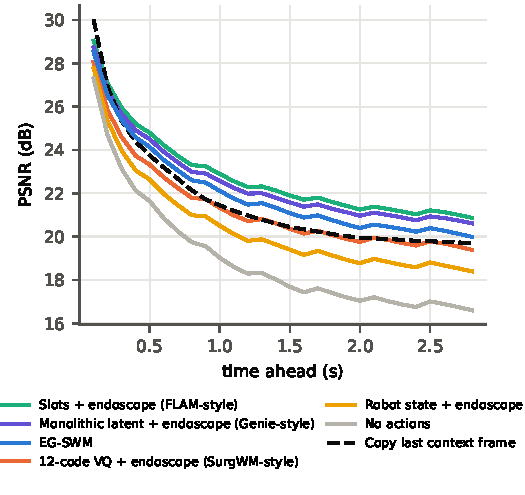
\includegraphics[width=\columnwidth]{e1_horizon.pdf}
\caption{PSNR of each predicted frame, 0.1--2.8\,s after the last context frame (mean over the \val{main/n_windows} test windows).}
\label{fig:horizon}
\end{figure}

\subsection{Fidelity}
Table~\ref{tab:main} compares the interfaces on \val{main/n_windows} windows spread evenly over the test cases. Paired over the same windows, \method{} improves on copying the last context frame by \val{diff/S_arms-copy_last/psnr}\,dB PSNR (95\,\% case-bootstrap interval \val{diff/S_arms-copy_last/psnr_ci}, \val{diff/S_arms-copy_last/wins} of \val{main/n_cases} cases) and \val{diff/S_arms-copy_last/ssim} SSIM, but is \val{diff/S_arms-copy_last/lpips} LPIPS worse: it trails the copied frame in the first \val{horizon/trail}\,s and leads by \val{horizon/lead}\,dB from 0.5\,s to the end of the 2.8\,s horizon. Replaying the inferred actions is worth \val{main/S_arms/delta_psnr}\,dB over the actions of another window, and the same model trained without actions is \val{diff/S_arms-S_none/psnr}\,dB \val{diff/S_arms-S_none/psnr_ci} worse, in \val{diff/S_arms-S_none/wins} of \val{main/n_cases} cases.

\subsection{Fidelity and control pull apart}
The interfaces whose learned action covers the whole frame give the best fidelity (Table~\ref{tab:main}): slot actions improve on \method{} by \val{diff/S_slots-S_arms/psnr}\,dB PSNR \val{diff/S_slots-S_arms/psnr_ci} (in \val{diff/S_slots-S_arms/wins} of the \val{main/n_cases} test cases) and the monolithic latent action by \val{diff/S_global-S_arms/psnr}\,dB \val{diff/S_global-S_arms/psnr_ci} (\val{diff/S_global-S_arms/wins} of \val{main/n_cases}), and adding a scene action, pooled outside every arm region, to \method{} improves \val{diff/S_arms_scene-S_arms/wins} of \val{main/n_cases} cases by \val{diff/S_arms_scene-S_arms/psnr}\,dB \val{diff/S_arms_scene-S_arms/psnr_ci} while making the arm actions more local (ratio \val{ctl/S_arms_scene/locality}) and lowering hallucinations to \val{ctl/S_arms_scene/halluc}\,\%. All three take over the endoscope: with the learned actions zeroed, a commanded endoscope motion is realised at \val{ctl/S_slots/gain_range}\,\% of its magnitude with slots, \val{ctl/S_global/gain_range}\,\% with the monolithic action and \val{ctl/S_arms_scene/gain_range}\,\% with the scene action, against \val{ctl/S_arms/gain_range}\,\% for \method{}. On the validation windows, another clip's endoscope action raises the replay error of the slot model by only \val{use/S_slots/cam_swap}\,\% (\method{}: \val{use/S_arms/cam_swap}\,\%), and the monolithic model is as faithful without an endoscope action as with it (difference \val{diff/S_global_nocam-S_global/psnr}\,dB \val{diff/S_global_nocam-S_global/psnr_ci}). At $\tau=0.9$, another clip's slot or monolithic action raises the flow-matching loss as much outside the arm regions as inside (slots +\val{use/S_slots/swap_t9_out}\,\% and +\val{use/S_slots/swap_t9_in}\,\%, monolithic +\val{use/S_global/swap_t9_out}\,\% and +\val{use/S_global/swap_t9_in}\,\%; \method{}'s arm actions +\val{use/S_arms/swap_t9_out}\,\% and +\val{use/S_arms/swap_t9_in}\,\%), so these actions steer no particular instrument. In a 12k-step pilot, the scene action carried as much endoscope motion when it was inferred from latents aligned by the measured endoscope motion, so it does not simply copy the motion it sees. We hypothesise that it describes content the context cannot predict, such as tissue entering the field of view, whose position reveals the motion; this remains to be tested directly. Under action replay, an action inferred from the real future can carry how that future looks, and the more of the frame it covers, the more it carries.

Among the interfaces that keep the endoscope controllable, \method{} is the most faithful by a wide margin: it leads the 12-code VQ action of SurgWM~\cite{surgwm} by \val{diff/S_arms-S_global_vq/psnr}\,dB \val{diff/S_arms-S_global_vq/psnr_ci} (in \val{diff/S_arms-S_global_vq/wins} of \val{main/n_cases} cases) and robot-state tokens with the endoscope action by \val{diff/S_arms-S_state/psnr}\,dB \val{diff/S_arms-S_state/psnr_ci} (\val{diff/S_arms-S_state/wins} of \val{main/n_cases}). The VQ action carries little (another clip's code raises the replay error by \val{use/S_global_vq/swap}\,\%), and its model falls below the copied frame (\val{diff/S_global_vq-copy_last/psnr}\,dB \val{diff/S_global_vq-copy_last/psnr_ci}). \method{} is thus the only interface that steers each instrument and the endoscope and still improves on the copied frame. Since none of the frame-wide actions has a physical controller that could set it in a simulation, \method{} keeps every learned action bound to an arm.

The gap in fidelity is concentrated where the arm actions cannot act (Table~\ref{tab:binding}). A mounted instrument has an image region in \val{bind/steps}\,\% of the latent steps of the test windows; \val{bind/none}\,\% of the mounted instruments have none in their window, being out of view, occluded, missed by the detector or not matched to the robot log, and \val{bind/some}\,\% have one in some steps only. In the \val{bind/n/two} test windows (of \val{main/n_windows}) in which at least two mounted instruments are bound for most of the horizon, \method{} trails the monolithic latent by \val{bind/two/S_global-S_arms}\,dB and the slots by \val{bind/two/S_slots-S_arms}\,dB. In the \val{bind/n/none} windows in which none is bound, it trails them by \val{bind/none/S_global-S_arms} and \val{bind/none/S_slots-S_arms}\,dB and falls below the copied frame. The frame-wide actions do not depend on the binding and describe whatever moves instead, so a higher binding coverage could narrow the gap without a frame-wide action.

\begin{table}[t]
\centering
\caption{PSNR on the \val{main/n_windows} test windows grouped by how many mounted instruments are bound to an arm region for most of the predicted steps.}
\label{tab:binding}
\resizebox{\columnwidth}{!}{\begin{tabular}{lccc}
\toprule
 & \multicolumn{3}{c}{Instruments bound (windows)} \\
\cmidrule(lr){2-4}
Model & none (93) & one (179) & $\geq$2 (728) \\
\midrule
Copy last context frame & 23.79 & 20.68 & 21.54 \\
None (unconditional) & 20.27 & 18.08 & 19.01 \\
Robot state & 20.63 & 18.28 & 19.37 \\
Robot state + camera & 22.36 & 19.53 & 20.42 \\
Monolithic latent (Genie) & 24.97 & 21.59 & 22.39 \\
Monolithic latent + camera & 25.10 & 21.58 & 22.35 \\
Monolithic VQ + camera (SurgWM-style) & 23.73 & 20.36 & 21.23 \\
Slots + camera (FLAM-style) & 25.32 & 21.85 & 22.67 \\
EG-SWM, no camera action & 20.11 & 20.42 & 21.96 \\
EG-SWM & 22.94 & 20.83 & 22.17 \\
EG-SWM + scene action & 24.56 & 21.27 & 22.37 \\
\bottomrule
\end{tabular}
}
\end{table}

\subsection{What each part of \method{} adds}\label{sec:parts}
The endoscope action is worth \val{diff/S_arms-S_arms_nocam/psnr}\,dB \val{diff/S_arms-S_arms_nocam/psnr_ci} to \method{}, in \val{diff/S_arms-S_arms_nocam/wins} of \val{main/n_cases} cases. Without it, the arm actions take on part of the frame-wide motion (at $\tau=0.9$, another clip's arm actions raise the loss outside the arm regions by \val{use/S_arms_nocam/swap_t9_out}\,\% instead of \val{use/S_arms/swap_t9_out}\,\%) and become less local (ratio \val{ctl/S_arms_nocam/locality} instead of \val{ctl/S_arms/locality}). Learned arm actions are worth \val{diff/S_arms_nocam-S_state_nocam/psnr}\,dB \val{diff/S_arms_nocam-S_state_nocam/psnr_ci} over robot-state tokens, both without the endoscope action. The state tokens alone add \val{diff/S_state_nocam-S_none/psnr}\,dB \val{diff/S_state_nocam-S_none/psnr_ci} over unconditional prediction and lower hallucinations from \val{ctl/S_none/halluc}\,\% to \val{ctl/S_state_nocam/halluc}\,\%; with them, the endoscope action is worth \val{diff/S_state-S_state_nocam/psnr}\,dB \val{diff/S_state-S_state_nocam/psnr_ci} and is realised at \val{ctl/S_state/gain_range}\,\% of its magnitude.

Grounding is what makes the arm actions local. When each arm's inverse-dynamics head and its input to the forward decoder cover the whole frame instead of the arm's instrument region, with one action per arm still bound through the robot log, fidelity barely changes (\val{diff/S_arms_poolglobal-S_arms/psnr}\,dB \val{diff/S_arms_poolglobal-S_arms/psnr_ci} better than \method{}, which leads in \val{diff/S_arms_poolglobal-S_arms/losses} of \val{main/n_cases} cases), but the locality ratio falls from \val{ctl/S_arms/locality} to \val{ctl/S_arms_poolglobal/locality}, \val{derived/pool_way}\,\% of the way to the monolithic action (\val{ctl/S_global/locality}), and the endoscope gain from \val{ctl/S_arms/gain} to \val{ctl/S_arms_poolglobal/gain}.

The forward decoder keeps the arm actions in use. Trained on the diffusion loss alone, only \val{use/S_arms_nofwd/active} of the 8 dimensions of each arm action stay active (KL \val{use/S_arms_nofwd/kl} instead of \val{use/S_arms/kl}\,nats per arm), another window's arm actions raise the replay error by \val{use/S_arms_nofwd/swap}\,\% instead of \val{use/S_arms/swap}\,\%, and replaying the inferred actions is worth \val{main/S_arms_nofwd/delta_psnr} instead of \val{main/S_arms/delta_psnr}\,dB over the actions of another window. The decoder improves fidelity by \val{diff/S_arms-S_arms_nofwd/psnr}\,dB PSNR \val{diff/S_arms-S_arms_nofwd/psnr_ci}, in \val{diff/S_arms-S_arms_nofwd/wins} of \val{main/n_cases} cases, and lowers FVD from \val{main/S_arms_nofwd/fvd} to \val{main/S_arms/fvd}, while the endoscope action is realised about as well without it (mean gain \val{ctl/S_arms_nofwd/gain} against \val{ctl/S_arms/gain}).

\begin{table*}[t]
\centering
\caption{Action-conditioned prediction on held-out SurgVU test cases (\val{main/n_cases} cases, 2.8\,s horizon, action replay, 50 Euler steps). PSNR, SSIM and LPIPS are means over cases with 95\,\% case-bootstrap intervals. Cam.\ gain: realised/commanded endoscope motion; Locality: share of the change inside the replaced arm's region over its area share; Halluc.: generated instruments not mounted per the robot log. \todo{ablation rows (whole-frame pooling, no forward decoder, wrong arm binding, console readout) as their runs finish}}
\label{tab:main}
\resizebox{\textwidth}{!}{\begin{tabular}{lcccccccc}
\toprule
Model & PSNR$\uparrow$ & SSIM$\uparrow$ & LPIPS$\downarrow$ & FVD$\downarrow$ & $\Delta$PSNR$\uparrow$ & Cam. gain$\uparrow$ & Locality$\uparrow$ & Halluc.$\downarrow$ \\
\midrule
Copy last context frame & 21.60\,{\scriptsize[20.94, 22.27]} & 0.681\,{\scriptsize[0.663, 0.699]} & 0.156\,{\scriptsize[0.145, 0.167]} & 653 & -- & -- & -- & -- \\
VAE reconstruction (ceiling) & 34.29\,{\scriptsize[33.97, 34.61]} & 0.949\,{\scriptsize[0.946, 0.952]} & 0.018\,{\scriptsize[0.017, 0.018]} & 22 & -- & -- & -- & 0.053 \\
Real frames (detector floor) & -- & -- & -- & -- & -- & -- & -- & 0.053 \\
None (unconditional) & 18.96\,{\scriptsize[18.49, 19.47]} & 0.583\,{\scriptsize[0.568, 0.599]} & 0.249\,{\scriptsize[0.238, 0.261]} & 422 & 0.00 & -- & -- & 0.130 \\
Robot state + camera & 20.44\,{\scriptsize[19.89, 21.01]} & 0.652\,{\scriptsize[0.636, 0.669]} & 0.206\,{\scriptsize[0.194, 0.218]} & 266 & 1.42 & 0.79 & -- & 0.078 \\
Monolithic latent + camera & 22.47\,{\scriptsize[21.94, 23.01]} & 0.703\,{\scriptsize[0.688, 0.718]} & 0.154\,{\scriptsize[0.145, 0.164]} & 180 & 3.17 & 0.16 & 1.46 & 0.074 \\
Monolithic VQ + camera (SurgWM-style) & 21.30\,{\scriptsize[20.76, 21.86]} & 0.671\,{\scriptsize[0.655, 0.687]} & 0.183\,{\scriptsize[0.172, 0.194]} & 206 & 2.11 & 0.81 & 1.53 & 0.082 \\
Slots + camera (FLAM-style) & 22.77\,{\scriptsize[22.24, 23.31]} & 0.713\,{\scriptsize[0.698, 0.727]} & 0.149\,{\scriptsize[0.139, 0.158]} & 169 & 3.55 & 0.05 & 1.44 & 0.078 \\
EG-SWM, no camera action & 21.52\,{\scriptsize[20.90, 22.15]} & 0.672\,{\scriptsize[0.654, 0.691]} & 0.176\,{\scriptsize[0.164, 0.189]} & 215 & 2.27 & -- & 2.02 & 0.080 \\
EG-SWM & 22.00\,{\scriptsize[21.43, 22.62]} & 0.691\,{\scriptsize[0.675, 0.708]} & 0.164\,{\scriptsize[0.153, 0.175]} & 186 & 2.78 & 0.70 & 2.42 & 0.076 \\
EG-SWM + scene action & 22.38\,{\scriptsize[21.82, 22.95]} & 0.701\,{\scriptsize[0.685, 0.717]} & 0.156\,{\scriptsize[0.146, 0.167]} & 174 & 3.04 & 0.22 & 3.50 & 0.072 \\
\bottomrule
\end{tabular}
}
\end{table*}

\section{Discussion and Limitations}\label{sec:discussion}
\todo{To be written with the results.} Planned points: what embodiment grounding buys and where it fails (occluded or out-of-view instruments, detector errors, stale log intervals); the porcine training-laboratory domain and transfer to clinical video; the absence of tissue-level physical guarantees; the use of world models for evaluation rather than control of real procedures.

\section{Conclusion}
\todo{To be written.}

\section*{Data and Code Availability}
Code, configurations, the case-level split and the evaluation windows: \url{https://github.com/GIND123/Surgical-World-Model}. Model weights (CC BY-NC-SA 4.0): \url{https://huggingface.co/GOVINDFROM/surgical-world-model}. SurgVU \cite{surgvu} is distributed by its organisers for non-commercial research; JIGSAWS \cite{jigsaws} requires a data-use agreement; the Open-H-Embodiment subsets \cite{openh} are released under CC BY 4.0, SAR-RARP50 \cite{sarrarp} under CC BY-NC-SA 4.0, and AutoLaparo \cite{autolaparo} on request for non-commercial use. No patient data were collected for this work.


\bibliographystyle{IEEEtran}
\bibliography{arxiv,manual}
\end{document}
